\documentclass[a4paper,onecolumn,10pt]{article}
\usepackage[polish]{babel}
\usepackage[utf8]{inputenc}
\usepackage[T1]{fontenc}
\usepackage[left=2.1cm,right=2.1cm]{geometry}
\usepackage[dvipsnames]{xcolor}
\usepackage{amsmath,calc,indentfirst,fancyhdr,amsfonts,graphicx,epstopdf,caption, mathcomp, subcaption,wrapfig, siunitx,pbox,float,algorithm}
\usepackage[noend]{algpseudocode}


\makeatletter
\def\BState{\State\hskip-\ALG@thistlm}
\renewcommand{\ALG@name}{Algorytm}
\makeatother

\renewcommand{\baselinestretch}{1.1}	 % odstep miedzy liniami
\addto\captionspolish{\renewcommand{\figurename}{Wykres}} % zmiana podpisu pod obrazkami, zamiast "Rysunek" bedzie "Wykres"
\newcommand{\NN}{\mathbb{N}}			 % makro do znaku liczb naturalnych

\newcommand{\R}[1]{\textcolor{red}{#1}}  % makro do polecenia z parametrami - tutaj 1 parametr
\newcommand{\G}[1]{\textcolor{green}{#1}} 
\newcommand{\B}[1]{\textcolor{RoyalBlue}{#1}} 
% kolorowanie {\B{argument}}

\newcommand{\PICTURES}{} % szybsza kompilacja dzieki stalej "usuwajacej" obrazki
						 % zakomentowanie \PICTURES powoduje znikniecie obrazkow

\pagestyle{fancy} % formatuj caly dokument
\fancyhead{}
\fancyfoot{}
\renewcommand{\headrulewidth}{0pt}
\fancyfoot[R]{\thepage} % dla stron poza tytulowa nr w prawym dolnym rogu

\fancypagestyle{plain}{ % dla strony tytulowej nr w prawym dolnym rogu
	
	\renewcommand{\headrulewidth}{0pt}
	\fancyhf{}
	\fancyfoot[R]{\thepage}
}
% 17 linia w preamble.tex

\renewcommand{\arraystretch}{1.2}

\title{\Large\vspace{-2.5cm}{\Huge S}PRAWOZDANIE - LABORATORIUM NR {\Huge7}\\
	\textbf{Interpolacja Lagrange'a z optymalizacją położeń węzłów} } 
\date{\Large11 kwietnia 2019}
\author{\Large Marek Kiełtyka}

\begin{document}
\maketitle
	
\vspace{-1.2cm}\section{Wstęp}
	
\subsection{Interpolacja}

Interpolacja polega na wyznaczeniu przybliżonych wartości funkcji w punktach niebędących węzłami (tj. punktami $ x_0,x_1,x_2,\dots,x_n \in [a,b] $ ) oraz na oszacowaniu ich błędu. Problem interpolacji można sprowadzić do znalezienia takiej funkcji interpolującej $F(x)$, która w węzłach przyjmuje takie same wartości jak badana funkcja $ y = f(x) $. Co ciekawe, nie jest konieczna znajomość funkcyjnej postaci $ f $ interpolowanej.

\subsubsection{Zastosowanie}

Dla zawartych w tablicy określonych położeń węzłów i wartości funkcji poszukuje się przybliżeń funkcji pomiędzy węzłami, co pozwala szybciej rozwiązywać równania nieliniowe. Interpolacja umożliwia lokalnie przybliżyć dowolną funkcję (nawet o bardzo skomplikowanej postaci) wielomianem, co ułatwia analizę rozwiązań np. w modelach fizycznych. Można ją również wykorzystać do całkowania numerycznego lub modelowania powierzchni w dwóch i trzech wymiarach.
\subsubsection{Interpolacja Lagrange'a}

Idea polega na znalezieniu wielomianu postaci
\begin{equation}
W_n(x) = a_0 + a_1x + a_2x^2 + \dots + a_nx^n
\end{equation}
poprzez rozwiązanie macierzowo układu równań liniowych
\begin{equation}
\begin{cases}
	a_0 + a_1x_0 + a_2x_0^2 + \dots + a_nx_0^n = y_0\\
	a_0 + a_1x_1 + a_2x_1^2 + \dots + a_nx_1^n = y_1 \\
	\vdots \\
	a_0 + a_1x_n + a_2x_n^2 + \dots + a_nx_n^n = y_n \\
\end{cases}
\end{equation}
w poszukiwaniu współczynników $$ a_i \mbox{ dla } i = 0,1,\dots,n $$ i dokonaniu odpowiednich przekształceń. Finalnie otrzymuje się
\begin{equation}
W_n(x) = \sum_{j=0}^{n} \left(y_j \prod_{k = 0 \wedge k \neq j}^n\frac{x - x_k}{x_j - x_k} \right).
\label{wzor}
\end{equation}

\subsection{Efekt Rungego}

Objawia się pogorszeniem jakości interpolacji wielomianowej  mimo zwiększania liczby węzłów. Najczęściej początkowy wzrost liczby węzłów interpolacji poprawia jej jakość, jednak przekroczenie pewnego poziomu powoduje znaczące pogorszenie rezultatów, co najczęściej uwidacznia się na końcach przedziałów interpolacji.

Zjawisko to jest typowe dla interpolacji za pomocą wielomianów wysokich stopni przy równoodległych węzłach. By go uniknąć, należy zastosować interpolację z węzłami bardzo gęsto umieszczonymi na krańcach przedziału, co wymusi częste przecinanie się wykresów funkcji interpolowanej i\,interpolującej.

\subsection{Poszukiwanie zer wielomianu Czebyszewa}

Aby zoptymalizować położenia węzłów, a w konsekwencji otrzymać lepsze dopasowanie, można skorzystać z szacowania położeń jako miejsc zerowych wielomianu Czebyszewa zgodnie z poniższym wzorem
\begin{equation}
x_m = \frac{1}{2}\left[(x_{max} - x_{min})cos\left(\pi\frac{2m + 1}{2n + 2}\right) + x_{min} + x_{max}\right]
\label{czeb}
\end{equation}
gdzie $ m = 0,1,\dots,n $, natomiast $ (n + 1) $ jest całkowitą liczbą węzłów oraz stopniem tego wielomianu.
		
\section{Zadanie do wykonania}

\subsection{Opis problemu}
	
Celem laboratorium było znalezienie wielomianu interpolacyjnego Lagrange’a $ W_n(x) $ dla funkcji: 
\begin{equation}
f(x) = e^{-x^2} \text{ w przedziale } x_{min} = -5, x_{max} = 5.
\label{funkcja}
\end{equation}
Zdefiniowano procedurę szacującą wartości funkcji w położeniach międzywęzłowych \textit{\begin{center}
		void interp(double x, const int n, double xNodes[], double yNodes[]),
\end{center}}gdzie 
\begin{itemize}
	\item $ x $ - położenie międzywęzłowe, w którym szukano przybliżonej wartości funkcji,
	\item $ n $ - stopień wielomianu interpolacyjnego,
	\item \textit{xNodes[]} - wektor węzłów $ x_m \text{ gdzie } m = 0,1,\dots,n $,
	\item \textit{yNodes[]} - wektor wartości funkcji $ f(x) $ w węzłach.
\end{itemize}
Ciało tej procedury było oparte na wzorze (\ref{wzor}), który to stosowano co krok równy $ 0,01 $ dla kolejnych położeń. Wcześniej, w celu poznania położeń węzłów równoodległych należało podzielić rozważany przedział o długości $$ x_{min} - x_{max} = 10 $$ na $ N $ podprzedziałów (przy czym pierwszy i ostatni węzeł wyznaczały krańce przedziału interpolacji). W drugiej części zadania do określania optymalnych położeń wykorzystano metodę znajdowania zer wielomianu Czebyszewa (\ref{czeb}). Otrzymane wyniki miały docelowo znaleźć się na wykresach obok przebiegu badanej funkcji (\ref{funkcja}) dla zmienianych stopni wielomianu $ n = \{5, 10, 15, 20\} $.

\newpage
\subsection{Wyniki}
	
\begin{figure}[h!]
	\begin{tabular}{cc}
		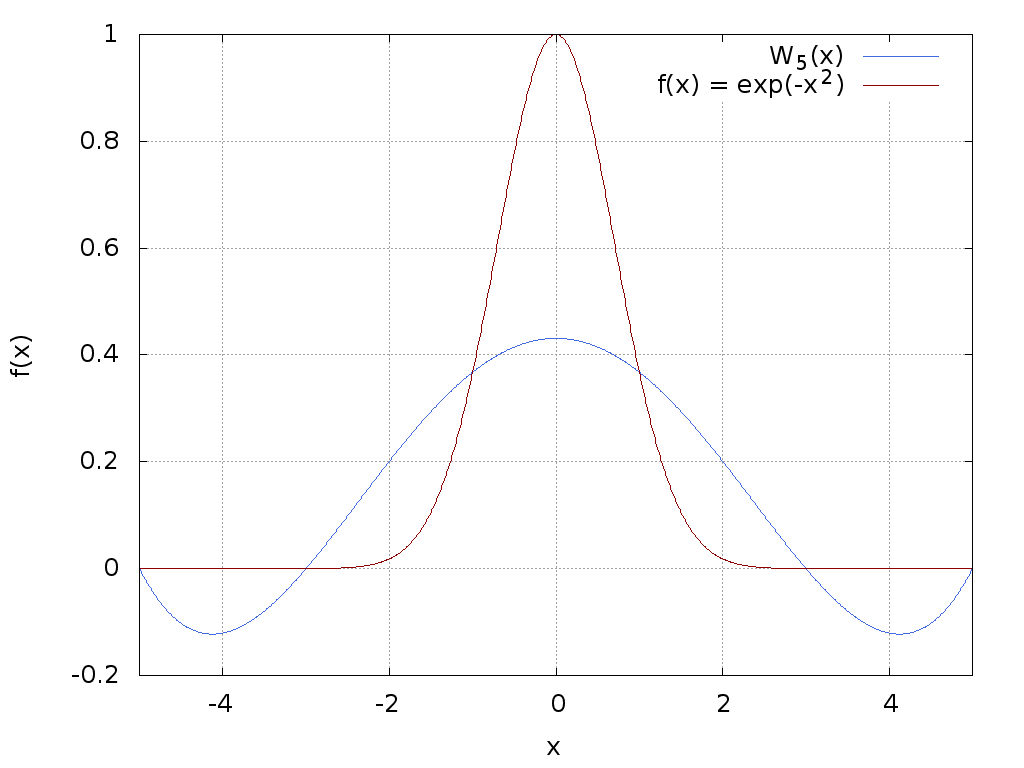
\includegraphics[width=75mm]{n5.png} &   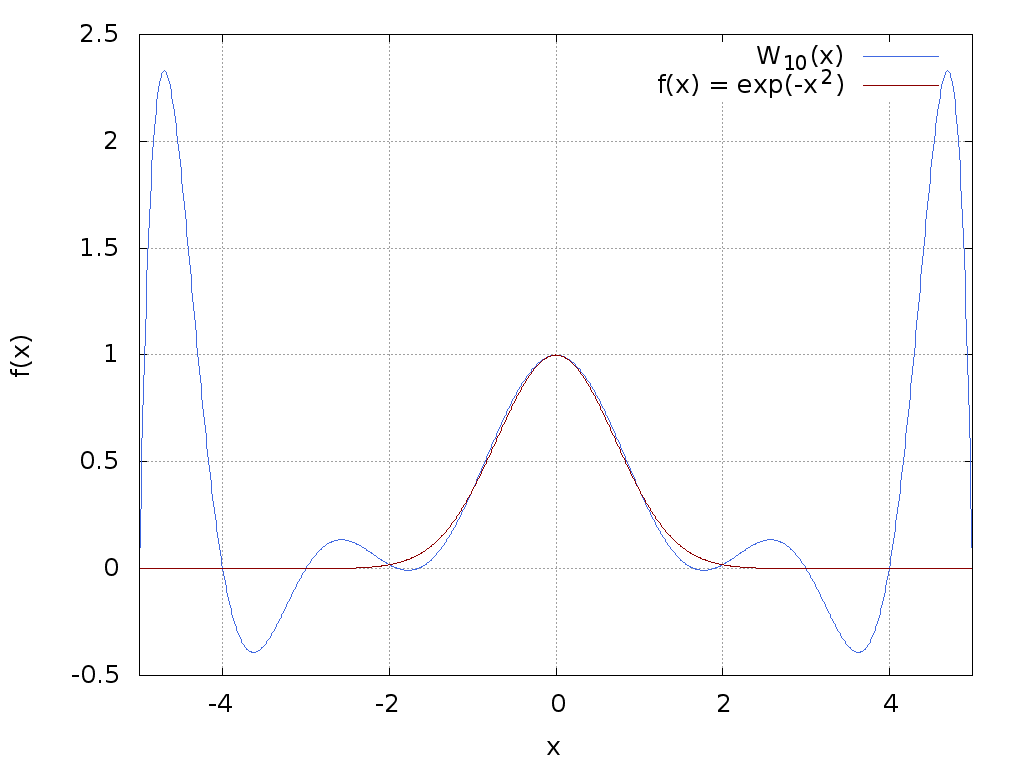
\includegraphics[width=75mm]{n10.png} \\
	$ n = 5 \implies \Delta x = 2 $ & $ n = 10 \implies \Delta x = 1 $ \\[6pt]
		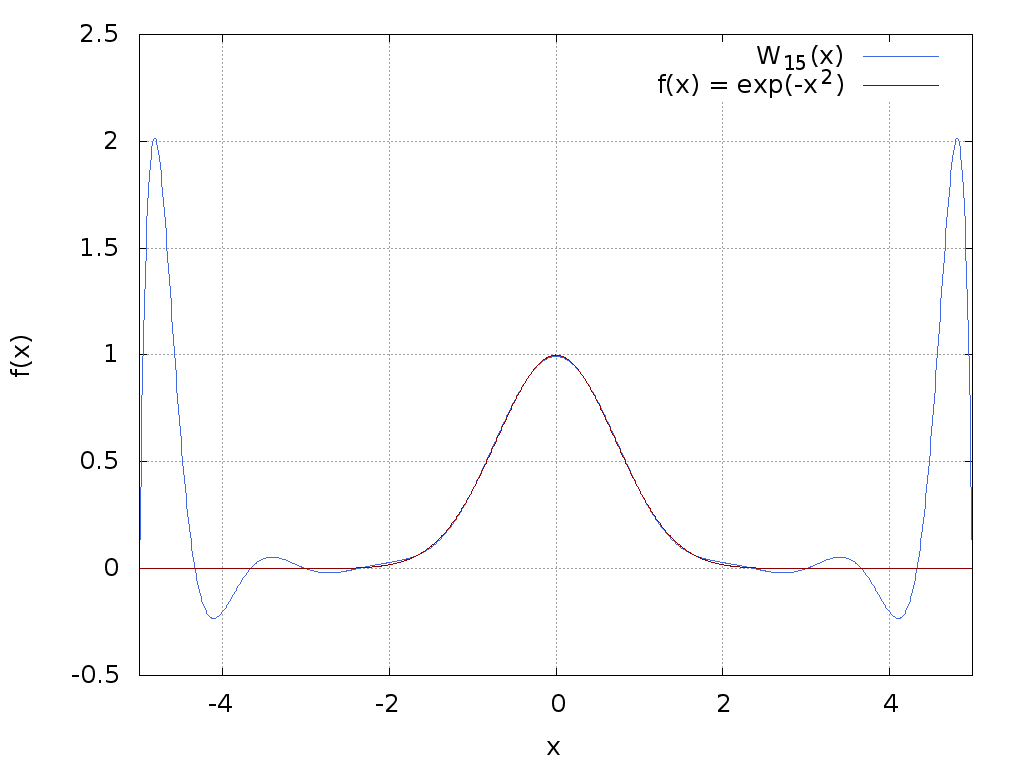
\includegraphics[width=75mm]{n15.png} &   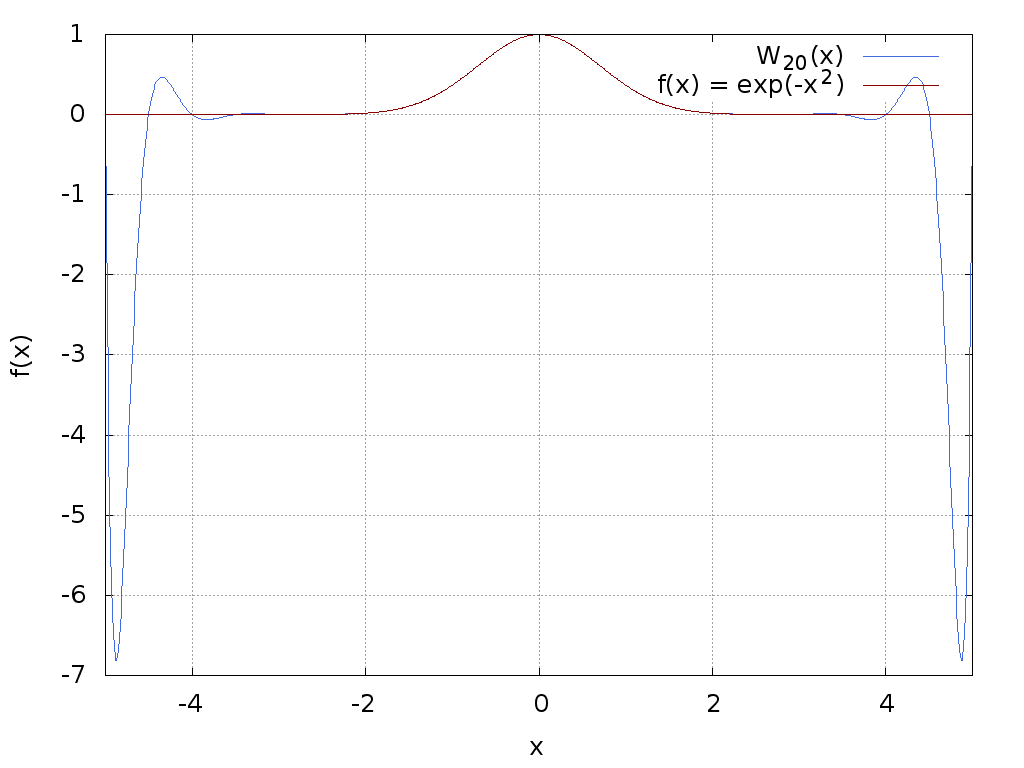
\includegraphics[width=75mm]{n20.png} \\
		$ n = 15 \implies \Delta x = \frac{2}{3} $ & $ n = 20 \implies \Delta x = \frac{1}{2} $ \\[6pt]
	\end{tabular}
	\caption{Wyniki interpolacji wielomianem Lagrange’a $ W_n(x) $ z równoodległymi węzłami. Węzły \newline o współrzędnych $ (x, f(x)) $ wyznaczają punkty przecięcia się obu wykresów. Liczba węzłów: $ n + 1 $.}
	\label{rowno}
\end{figure}
\begin{figure}[h!]
	\begin{tabular}{cc}
		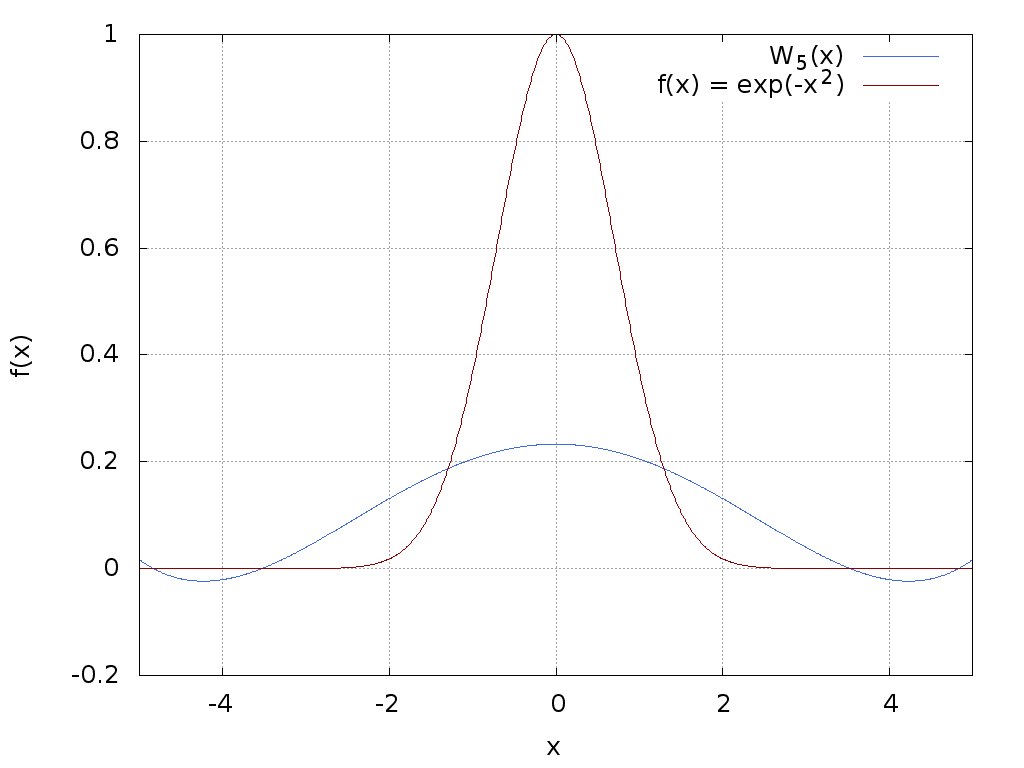
\includegraphics[width=75mm]{czeb_n5.png} &   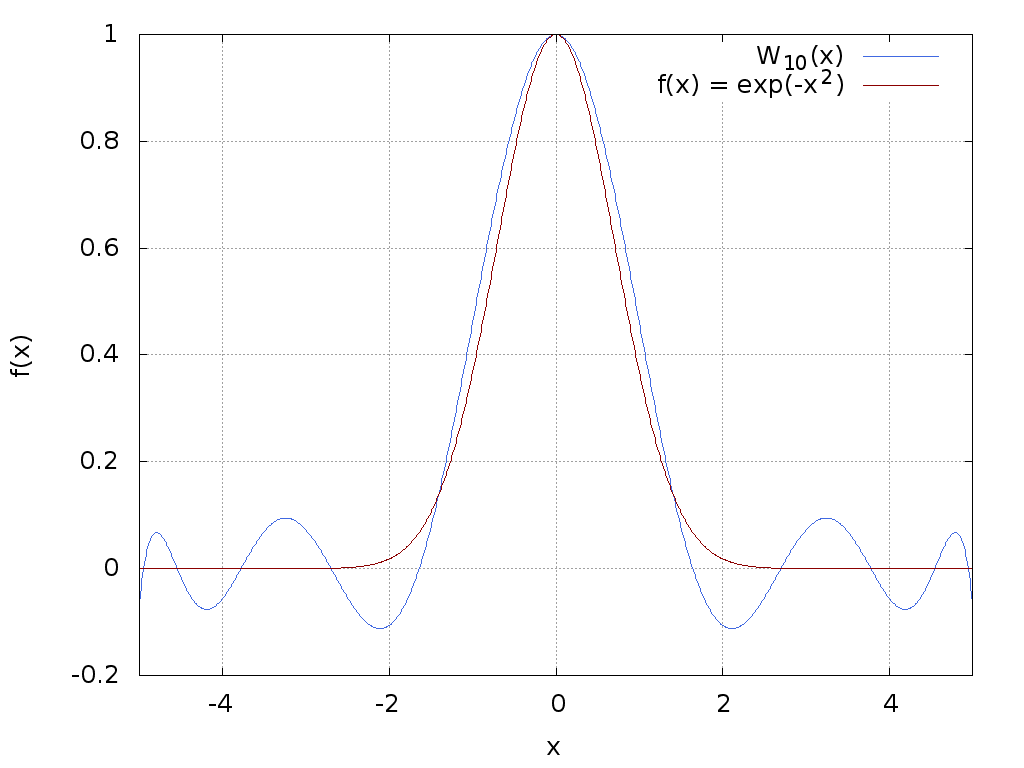
\includegraphics[width=75mm]{czeb_n10.png} \\
	$ n = 5 $ & $ n = 10 $ \\[6pt]
		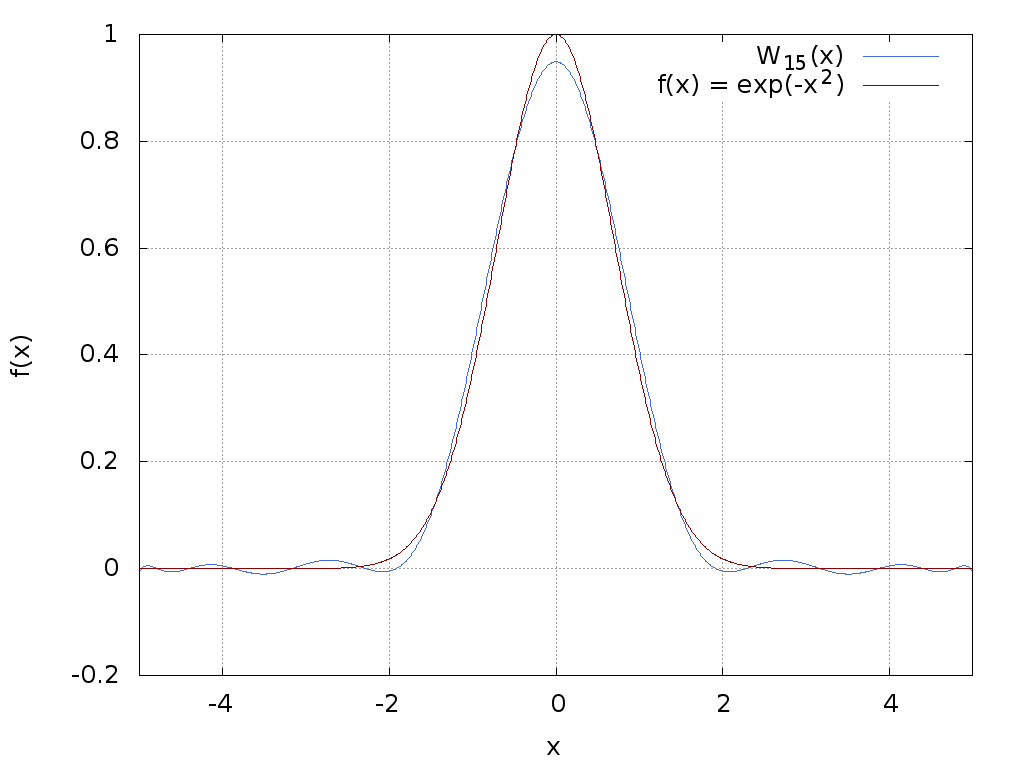
\includegraphics[width=75mm]{czeb_n15.png} &   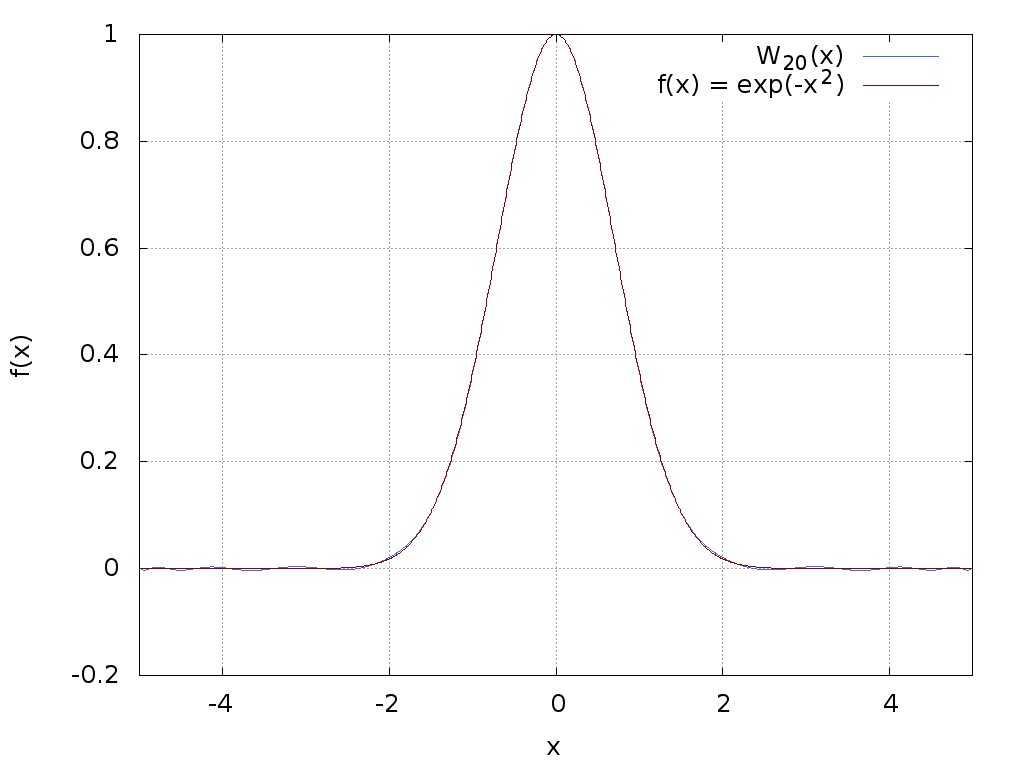
\includegraphics[width=75mm]{czeb_n20.png} \\
		$ n = 15 $ & $ n = 20 $ \\[6pt]
	\end{tabular}
	\caption{Wyniki interpolacji wielomianem Lagrange’a $ W_n(x) $ z węzłami, których współrzędne są wyznaczone przez miejsca zerowe wielomianów Czebyszewa. Węzły o współrzędnych $ (x, f(x)) $ wyznaczają punkty przecięcia się obu wykresów. Liczba węzłów: $ n + 1 $.}
	\label{czebyszew}
\end{figure}
	
\newpage
\section{Wnioski}
	
Wspólną cechą obu rysunków jest znacząca poprawa jakości interpolacji w miarę zwiększania liczby węzłów. Jak wyżej wspomniano (a potwierdzono wykonaniem zadania), wymusza to na wykresach częstsze ich wzajemne przecinanie, zatem dopasowanie musi być automatycznie lepsze.

Jednak dla rysunku (\ref{rowno}) obserwuje się propagację błędu szacowania na końcach przedziału interpolacji, co jest zgodne z efektem Rungego. Zmiana sposobu wyznaczania położeń węzłów na wykorzystanie wielomianu Czebyszewa skutkuje niemal idealnym dopasowaniem mimo stosunkowo wysokiego jego stopnia. Dla $ n = 20 $ uzyskano bardzo korzystne, niemal idealne pokrycie.

Przebiegi funkcji świadczą o poprawności przeprowadzonego rozumowania.
	
\end{document}